\section{Izboljšava algoritmov z vnosom človeških karakterističnih značilnosti}
Ljudje se lahko hitro naučimo novih konceptov iz nekaj pozitivnih slik, kar pa je za računalniški model zelo težavna naloga \cite{jia2013visual}. Naučene koncepte lahko fleksibilno uporabimo na različnih primerih, v drugačnem okolju, kar pa za algoritme ne velja \cite{lake2015human}. V ta namen je \citea{jia2013visual} predlagal nov izziv za strojno učenje---učenje vizualnih konceptov. V tem izzivu mora sistem določiti, če izbrana slika spada v določen koncept. 

\begin{figure}[!htbp]
	\centering
	\includegraphics[width=0.7\columnwidth]{jia_1}
	\caption{Slike iz \cite{deng2009imagenet}.}
\end{figure}

Problematiko so osvetlili s razvojem algoritma, ki bolje oponaša učenje otrok in se lahko nauči novih vizualnih konceptov iz majhnega števila slik. Algoritem temelji na linearnem logističnem regresorju z minibatch Adagrad algoritmom in posplošenim Bayesovim algoritmom. Regresor so učili na ImageNet 2010 podatkovni bazi. Z njim so dosegli \SI{41.28}{\%} top-1 natančnost in \SI{61.69}{\%} top-5 natančnost na testnih podatkih. Bayesov algoritem temelji na računanju verjetnosti, da slika iz neznane kategorije spada v kategorijo vzorčnih slik. Tu so uporabili konfuzijsko matriko, s katero so dodali vizualno nejasnost, ki se lahko pojavi zaradi nepopolnosti razvrščevalnikov.

Za testiranje svoje hipoteze so avtorji uporabili slike iz ImageNet 2010 podatkovne baze. Pri tem so izbrali $4$ tipe kategorij iz pomenskega drevesa. Prva kategorija je bila najbolj specifična (borovnica), nadaljnje pa so bile vedno bolj posplošene (sadje, rastlina). Pri izbiranju kategorij so pazili, da je pridobljena informacija med njimi največja. 

Podatke za referenco, so v \cite{jia2013visual} pridobili s pomočjo ljudi. Vsak subjekt so testirali tako, da so mu podali $5$ vzorčnih slik, ki naj bi predstavljale nek koncept. Subjekt je nato za novih $20$ slik ($12$ pravilnih in $8$ napačnih) moral določiti, ali so povezane z vzorčnimi slikami.

Z eksperimenti so pokazali, da dobijo za okoli \SI{10}{\%} boljše rezultate glede na ostale metode in ravno za toliko slabše rezultate glede na človeka. 



Problematiko učenja konceptov so opredelili tudi v delu \cite{lake2015human}. Razvili so novo metodo Bayesovega programskega učenja (BPL), ki se lahko nauči velika števila konceptov samo iz enega primera. Osnovni koncepti so predstavljeni kot verjetnostni programi, nove koncepte pa se BPL uči z združevanjem starih na podlagi vzročnosti in sestave objektov iz realnega sveta \cite{lake2015human}. 

\begin{figure}[!htbp]
	\centering
	\includegraphics[width=0.7\columnwidth]{lake_1}
	\caption{}
\end{figure}

BPL so preizkusili na ročno pisanih črkah, kjer so osnovne koncepte (primitive) predstavljale zaključene krivulje, ki jih naredimo s peresom, sestavo objektov pa so določili na podlagi prostorskih relacij med njimi. Algoritem so raziskovalci naučili tako, da so mu podali učno sliko ročno napisane črke, ta pa je s svojimi koncepti rekonstruiral črko, ki je bila najbolj verjeten približek. Naučeno strukturo je BPL nato uporabil kot osnovo za rekonstrukcijo testnih slik.

BPL algoritem so primerjali z rezultati $40$ ljudmi, ki so med testiranjem morali za vsak primer črke najti najbolj podobno izmed $20$ ponujenih. Raziskovalci so za BPL dobili podobno stopnjo napake, kot pri človeku, medtem ko so bile globoke nevronske mreže veliko slabše. Povzetek rezultatov iz \cite{lake2015human} je prikazan v tabeli \ref{tab:lake_1}. 

\begin{table}[!htbp]
	\centering
	\begin{tabular}{l S[table-format=1.3, round-mode=places, round-precision=2]}
		\toprule
		\textbf{Metoda} & \thead{Stopnja napake [\%]}  \\
		\midrule
		Ljudje & 4.5  \\
		BPL & 3.3 \\
		ConvNet & 13.5 \\
		SiameseNet & 8.0 \\
		\bottomrule
	\end{tabular}
	\caption{}
	\label{tab:lake_1}
\end{table}

Poleg primerjanja stopnje napake so v \cite{lake2015human} izvedli še poenostavljen Turingov test, kjer je posameznik poskušal razpoznati, katero črko je narisal človek in katero je generiral algoritem. Ljudje so razlike zelo težko razpoznali, kar nakazuje na približevanje BPL algoritma človeku. Seveda so \citea{lake2015human} poudarili, da BPL algoritem še vedno vsebuje slabše koncepte kot človek, saj strukture niso tako abstrakne in kompleksne, da bi jih lahko uporabili za razpoznavanje vsakodnevnih objektov, kot so vozila in drevesa.


V \cite{scheirer2014perceptual} so se izboljšanja modelov lotili z neposrednim koriščenjem človeške sposobnosti. S spletnim testiranjem ljudi so pridobili vzorce napak, ki so jih prevedli v človeške utežne funkcije. Te so nato uporabili v SVM, kjer funkcija dodaja kazni mejam, ki niso skladne s podatki o ljudeh.

\begin{figure}[!htbp]
	\centering
	\includegraphics[width=0.7\columnwidth]{scheirer_1}
	\caption{Slike iz \cite{jain2010fddb}.}
\end{figure}

Utežno funkcijo so pridobili s pomočjo dveh testov. V prvem testu so avtorji vsakemu merjencu $102\times$ pokazali $3$ slike, izmed katerih je merjenec moral izbrati sliko z obrazom. Pri tem so spreminjali območje vidnosti obraza. Tako so lahko dobili krivuljo človekove natačnosti glede na vidno območje obraza.

V drugem testu so uporabili sivinske slike, ki so se prikazale za \SI{50}{\ms}. Merjenec je moral nato določiti, ali je na sliki videl obraz ali ne.

\citea{scheirer2014perceptual} je z eksperimenti pokazal, da z uporabo take utežne funkcije močno izboljšamo delovanje detektorjev obraza. Izboljšavo lahko še povečamo če uporabimo značilke, ki temeljijo na biologiji (Cox in Pinto).

Avtorji dela \cite{fong2017using} so se koriščenja človeške sposobnosti lotili še bolj elementarno. Ti so v učni proces implementirali meritve človeških možganskih aktivnosti fMRI. Meritve so izvajali na enem merjencu, ko je ta opazoval vse slike iz izbrane podatkovne baze. Z merjenjem so dobili nevronski odziv na zazanavanje slike in jih uporabili kot značilke za učenje SVM razvrščevalnika z RBF jedrom. Rezultate razvrščanja so nato transformirali v verjetnosti preko logistične funkcije. Na ta način so dobili utežno funkcijo aktivnosti, s katero so kaznovali napačno razvrščanje pri učenju novih modelov.

\begin{figure}[!htbp]
	\centering
	\includegraphics[width=0.7\columnwidth]{fong_1}
	\caption{Avtor fMRI slike je \cite{kelley2009fmri} po licenci \url{https://creativecommons.org/licenses/by/2.0/legalcode}. Ostale slike smo dobili iz ImageNet podatkovne baze \cite{deng2009imagenet}.}
\end{figure}


Pri eksperimentiranju so uporabili podatkovno bazo \num{1386} naravnih prizorov ljudi, živali, zgradb, hrane in vozil. Za testiranje so uporabili SVM razvrščevalnik s RBF jedrom, ki so ga učili na HOG in CNN značilkah. CNN značilke so dobili iz prednaučenega AlexNet modela.

Njihovi eksperimenti so pokazali, da lahko s takim načinom izboljšamo delovanje razvrčevalnikov. Izboljšave so najbolj opazne na ročno izdelanih značilkah, kot je HOG.  

\citea{branson2010visual} je prav tako koristil človeške sposobnosti, vendar na popolnoma drugačen način. Sestavil je hibrid med modelom in človekom, ki ga imenujemo tudi človek-v-zanki (angl. Human-in-the-loop) \cite{branson2010visual}. Pri tem načinu, model uporabimo za razvrščanje enostavnih problemov, človeka pa za ostalo. Delovanje so prikazali na podatkovni bazi Birds-200, kjer s pomočjo razvrščevalnika in vprašanji, ki jih postavimo subjektu določimo kategorijo ptice, ki je prikazana na sliki. 

\begin{figure}[!htbp]
	\centering
	\includegraphics[width=0.7\columnwidth]{branson_1}
	\caption{Slike iz \cite{welinder2010caltech}.}
\end{figure}

V primeru, da so za razvrščanje ptic v kategorije uporabili samo vprašalnik, so ljudje, pred pravilnim razvrščanjem, v povprečju odgovorili na $12$ vprašanj. Ob pomoči računalniškega vida pa se je število vprašanj zmanjšalo na $7$. Gledano z druge perspektive je človek v povprečju povečal natančnost algoritma iz $\sim$\SI{19}{\%} na $\sim$\SI{66}{\%}. 

Dodajanje človeka za izboljšanje sistema so raziskovali tudi v \cite{mottaghi2013analysing}. Tu so se osredotočili na CRF modele s katerimi izvajamo segmentacijo, detekcijo, analizo oblike, razpoznavanje prizora in razumevanje konteksta. V raziskavi, v kateri je sodelovalo več kot $500$ oseb, so zamenjali različne segmente CRF modela s človekom in preizkusili njegovo delovanje na MSRC-21 podatkovni bazi. Rezultati so pokazali, da obstaja potencial izboljšanja modelov pri lokalni segmentaciji.

\begin{figure}[!htbp]
	\centering
	\includegraphics[width=0.7\columnwidth]{mottaghi_1}
	\caption{Slike iz MSRC podatkovne baze \cite{shotton2006textonboost}}
\end{figure}

Razširitev dela \cite{mottaghi2013analysing} so izvedli v \cite{mottaghi2016human}, kjer so se osredotočili na izboljšanje sistema detekcije objektov in razpoznavanja prizora. Sistem segmentacije so ponovno preizkusili na bolj zahtevni PASCAL podatkovni bazi in prišli do podobnih zaključkov. 


V delu  \cite{otoole2007fusing} so se raziskovalci osredotočili na združevanje človeka in algoritmov za razpoznavanje obrazov. Rezultate algoritma in ljudi so združili z regresijo delnih najmanjših kvadratov. Merjenci so v eksperimentu določevali verjetnost, da para slik predstavljata isto osebo. Slike so lahko opazovali \SI{2}{\s}. V eksperimentu je sodelovalo $49$ oseb (25 moških in 24 žensk). Tudi njihovi rezultati so pokazali, da združevanje pripomore k izboljšanju rezultatov. 

Zanimivo raziskavo so izvedli \citea{vondrick2015learning}, kjer so raziskovali pristranskost človeka v razpoznavanju objektov. Argumentirali so, da razlika v delovovanju algoritmov in človeka nastaja tudi zaradi človeške pristranskosti. Pokazali so, da pristranskost lahko v določeni meri ovrednotimo in jo tudi uporabimo za izboljšanje algoritmov. 

Pristranskost so določili tako, da so ljudem pokazali barvne slike belega šuma in jim naročili naj jih kategorizirajo v izbrane kategorije. Z velikim številom ljudi, ki so sodelovali na Amazon Mechanical Turk, so dobili povprečne slike, ki so nakazovale oblike, podobne izbranim kategorijam. Pridobljene slike so nato klasificirali in primerjali s testno množico realnih slik iz podatkovne baze PASCAL VOC 2011. Ugotovili so, da jih algoritmi lahko dobro klasificirajo, saj so bile povprečne natančnosti večje od naključnosti. Povprečne slike so \citea{vondrick2015learning} zato določili kot predloge človeške pristranskosti za izbrano kategorijo. 






